% calculus:x07 GDC:NO
\begin{question}
  \hspace*{\fill} [Note maximale: 16]\par
  \medskip
  \noindent La figure suivante représente une partie de la représentation graphique de la fonction $f(x) = 2x^2$.\par
  \medskip
  \begin{center}
    \noindent La figure n'est pas a l'échelle\par
    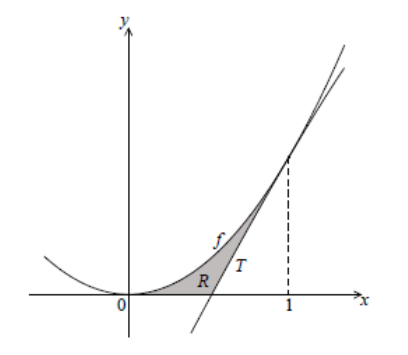
\includegraphics[scale=0.4]{temp_f_2xsquared}\par
  \end{center}
  \medskip
  \noindent La droite T est la tangente à la représentation graphique de $f$ en $x = 1$.\par
  \medskip
  (a) Montrez que l’équation de $T$ est $y = 4x - 2$.\hspace*{\fill} [5]\par
  \medskip
  (b) Trouvez l’abscisse à l’origine de $T$.\hspace*{\fill} [2]\par
  \medskip
  (c) La région grisée $R$ est limitée par la représentation graphique de $f$, la droite $T$ et l’axe des abscisses.\par
  \hspace{1em}(i)  Donnez une expression de l’aire de $R$.\par
  \hspace{1em}(ii) Trouvez l’aire de $R$.\hspace*{\fill} [9]\par
  \medskip
\end{question}


